\section{Introduction}
Let $\norm{\cdot} \colon \R^2 \to \R$ be a norm. Then we define the distance function as
\begin{equation}
    \dist(p, q) = \norm{p - q}.
\end{equation}
For $1 \leq p < \infty$ we define the $L^p$ norm by
\begin{equation}
    \norm{(x, y)}_p = {\big(\abs{x}^p + \abs{y}^p\big)}^{1/p},
\end{equation}
and we note that $\norm{ \cdot }_2$ is the well-known Euclidean distance. For $p = 1$, the above reduces to
\begin{equation}
    \norm{(x, y)}_1 = \abs{x} + \abs{y}.
\end{equation}
Letting $p \to \infty$, we also obtain the norm
\begin{equation}
    \norm{(x, y)}_{\infty} = \max\big(\abs{x}, \abs{y}\big).
\end{equation}
\begin{defn}[Voronoi diagram]
Let $P = \curly{p_1, p_2, \ldots, p_n} \subset \R^2$. The cells corresponding to each point are denoted by
\[
    \mathcal{V}(p_i) = \makeset{q \in \R^2}{\dist(q, p_i) < \dist(q, p_j) \text{ for all } i \ne j}.
\]
The Voronoi diagram of $P$, denoted $\Vor(P)$, is the subdivision of $\R^2$ consisting of the cells $\mathcal{V}(p_1), \mathcal{V}(p_2), \ldots, \mathcal{V}(p_n)$.
\end{defn}

The following figure shows how the Voronoi diagram for 9 random points looks like with regards to some different $L^p$ norms:

\begin{figure}[H]
    \centering
    \subfloat[$p = 1$]{
      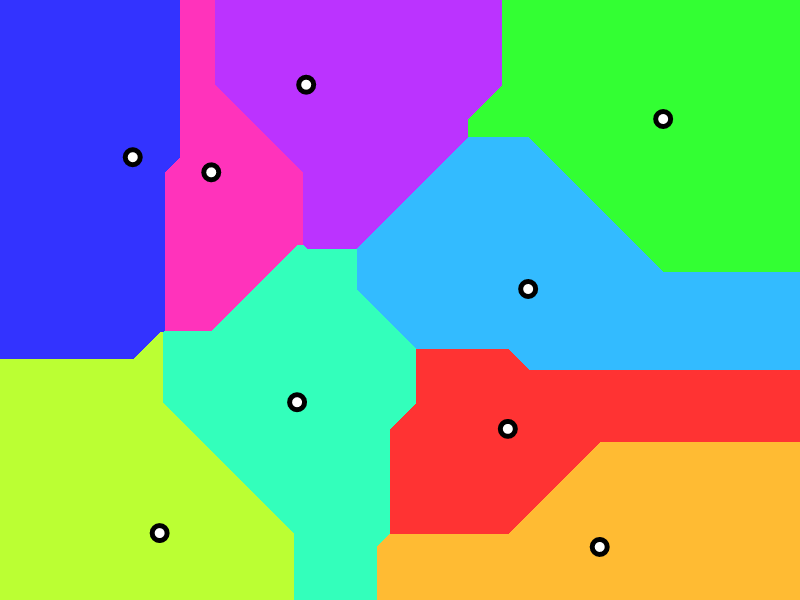
\includegraphics[scale=0.21]{naive-voronoi-L1}
    }
    \subfloat[$p = 2$]{
      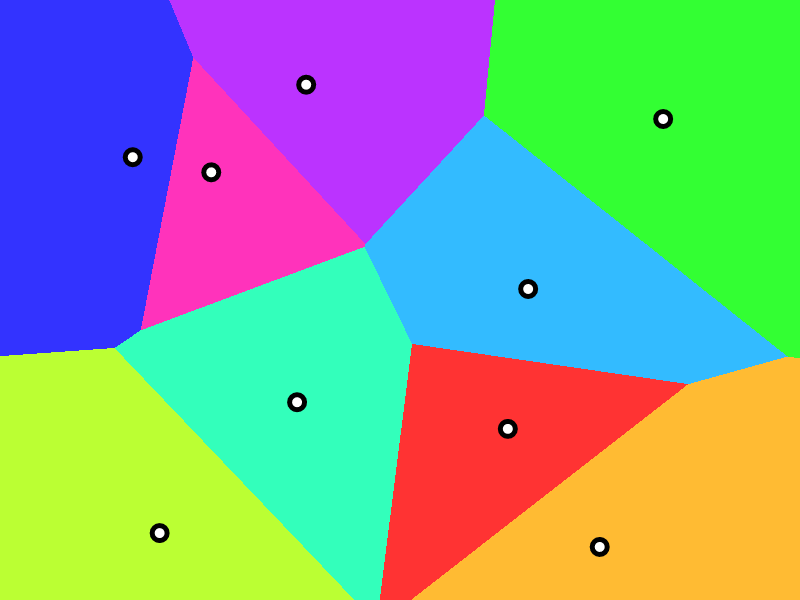
\includegraphics[scale=0.21]{naive-voronoi-L2}
    }
    \hspace{0mm}
    \subfloat[$p = 5$]{
      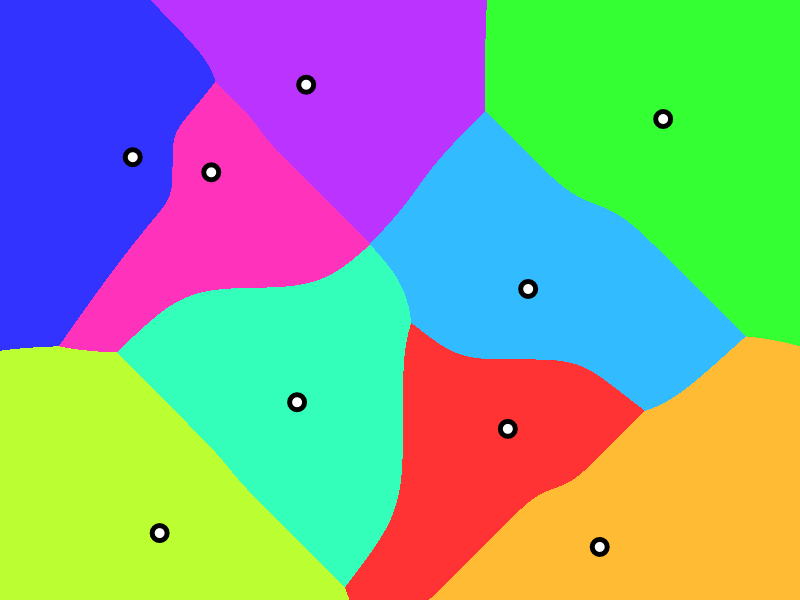
\includegraphics[scale=0.21]{naive-voronoi-L5}
    }
    \subfloat[$p = \infty$]{
      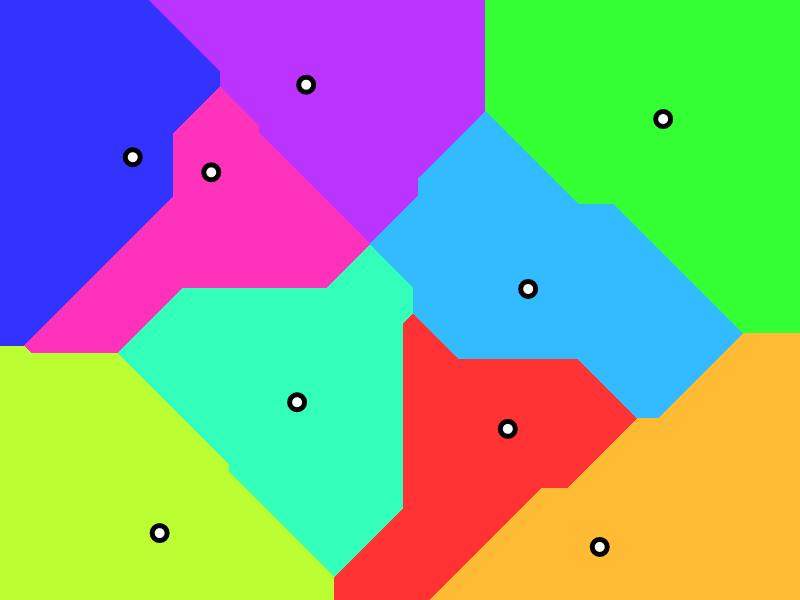
\includegraphics[scale=0.21]{naive-voronoi-Linfty}
    }
    \caption{$\Vor(P)$ of 9 random points using different $\norm{\,\cdot\,}_p$}
    \label{fig:naive-voronoi}
\end{figure}
The above figures were generated using a very naive algorithm, which for each each pixel determinates which of the 9 points is the closest with regards to the chosen norm. A demo is available in $\boxed{\textsf{demos/pixel-voronoi-naive}}$. \\

Note that some of the cells may be unbounded, for example the bottom left green cell in the above figure. For $p = 1$ and $p = \infty$ the boundaries of the cells $\mathcal{V}(p_i)$ are characterised by lines, rays and segments that can only point in the 8 compass directions. For $p = 2$ the boundaries consist of lines, rays and segments which can point in any direction. Interestingly, for $2 < p < \infty$ it seems that the boundary consists of smooth curves that are not necessarily part of a line. \\

We now want to look at the graph structure of the Voronoi diagram. For $P = \curly{p_1, p_2, \ldots, p_n} \subset \R^2$ the set
\[
    \VorG(P) = \R^2 - \bigcup_{i=1}^n \mathcal{V}(p_i)
    = \makeset{q \in \R^2}{\dist(q, p_i) = \dist(q, p_j) \text{ for some } i \ne j}
\]
turns out to be an embedding of a graph, where some of the edges are infinite, here's a visualization:
\begin{figure}[H]
    \centering
    \subfloat[$p = 1$]{
      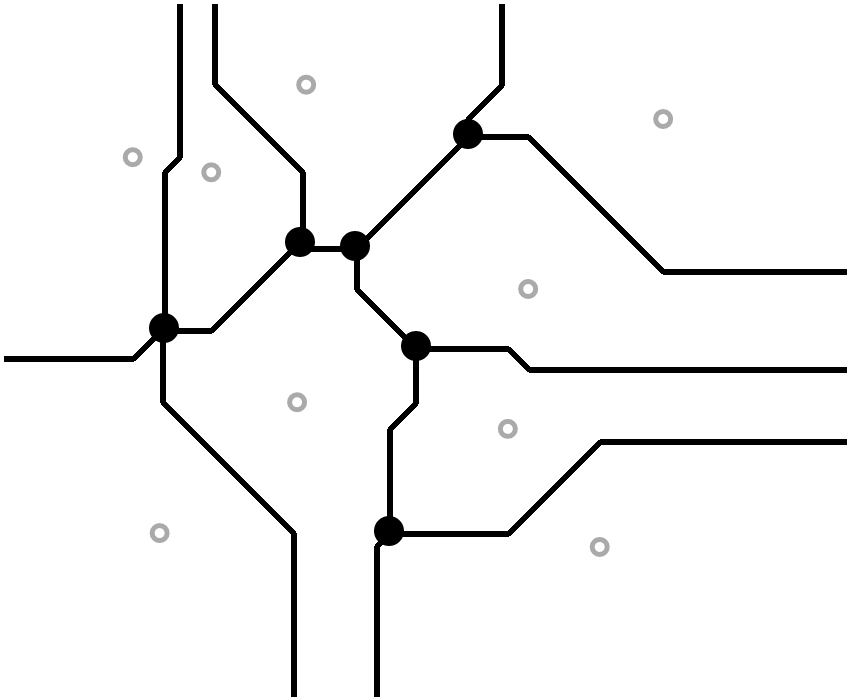
\includegraphics[scale=0.21]{naive-voronoi-graph-L1}
    }
    \subfloat[$p = 2$]{
      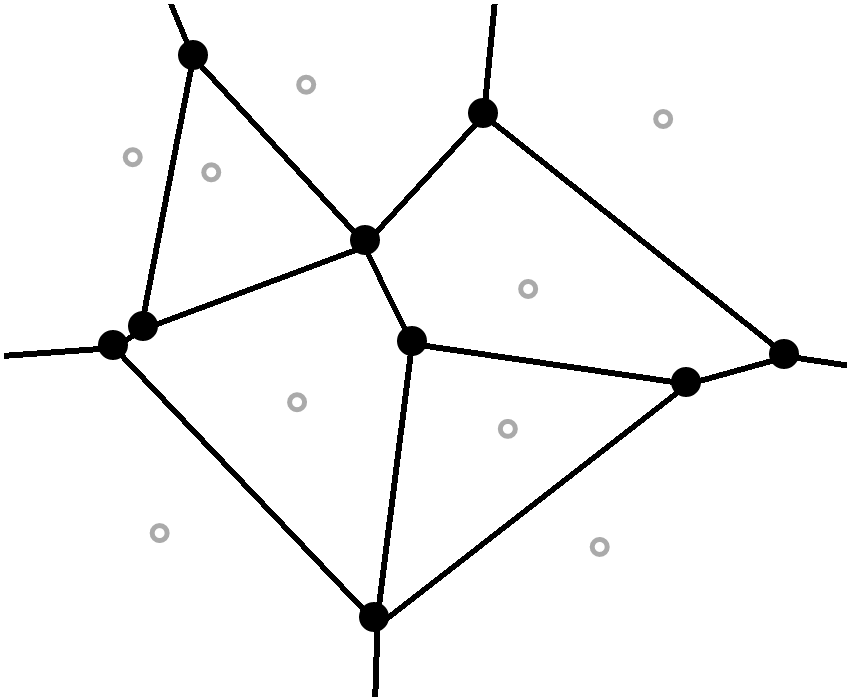
\includegraphics[scale=0.21]{naive-voronoi-graph-L2}
    }
    \hspace{0mm}
    \subfloat[$p = 5$]{
      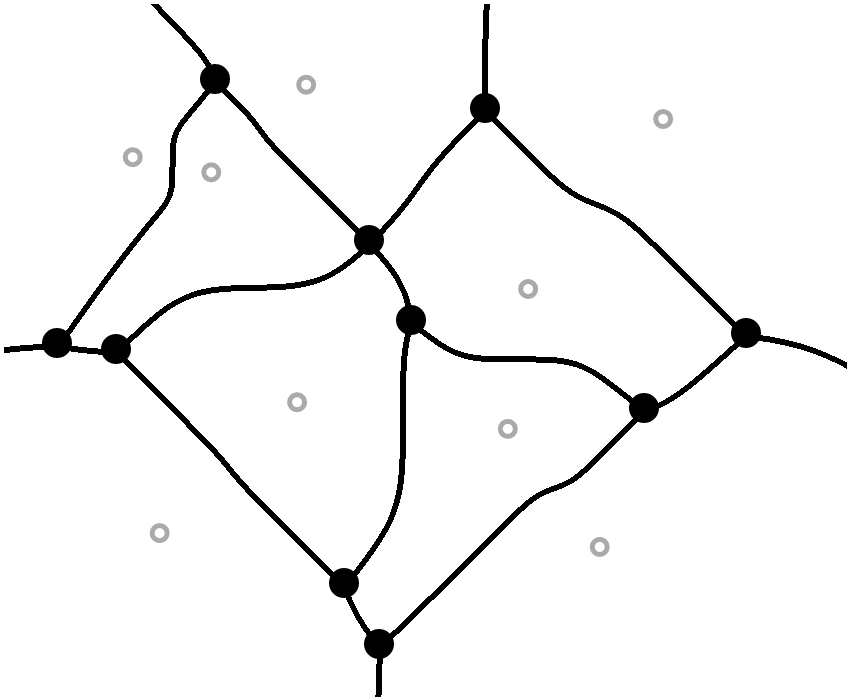
\includegraphics[scale=0.21]{naive-voronoi-graph-L5}
    }
    \subfloat[$p = \infty$]{
      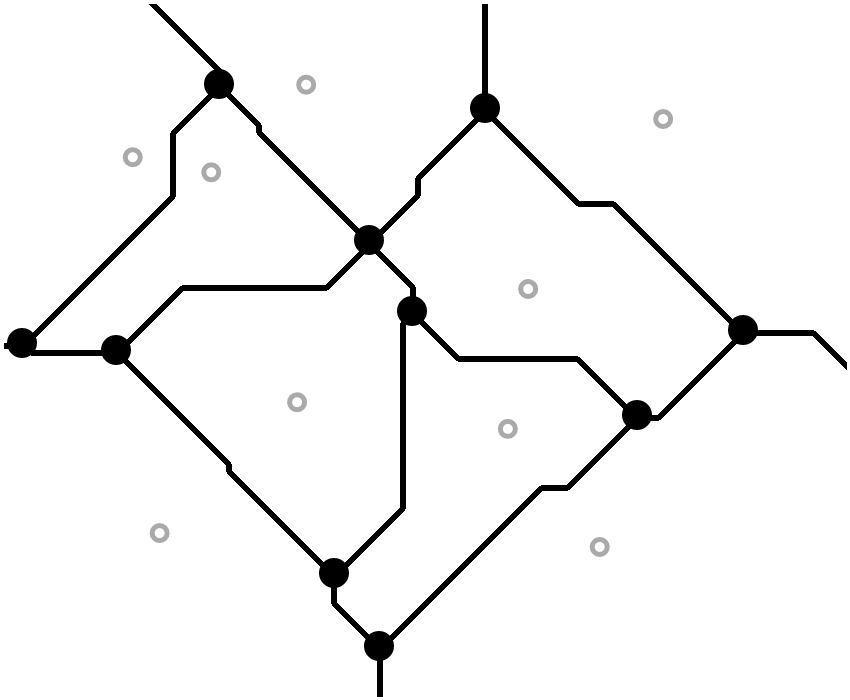
\includegraphics[scale=0.21]{naive-voronoi-graph-Linfty}
    }
    \caption{$\VorG(P)$ of the 9 random points using different $\norm{\,\cdot\,}_p$.}
\end{figure}
The above figures were generated by first generating the images from Figure \ref{fig:naive-voronoi} and then performing the following algorithm: For each pixel, we look at the surrounding pixels within a small disk about that point, and if it contains exactly 2 different colors, we know that we're looking at an edge, so we color the pixel black, and if we see 3 colors or more, we know that we're at a vertex. If we only see 1 color, then we just color the pixel white.

Note that it's the black vertices and edges which make up the graph, the gray points from $P$ are just there for visualization. Rather than computing $\Vor(P)$, our algorithms will actually compute $\VorG(P)$, and from there be able to compute $\Vor(P)$. \\

Now, a natural question arises: how do we store Voronoi diagrams? We'll need the following geometric data structure:
\begin{defn}[DCEL]
\todo{Define the DCEL.}
\end{defn}
Note that the DCEL does not support infinite edges, so what we do is put a bounding box $B$ with some padding around the vertices of $\Vor(P)$, and then intersect the infinite edges and faces with the boundary of $B$ and only keep the part inside the bounding box.
\[
    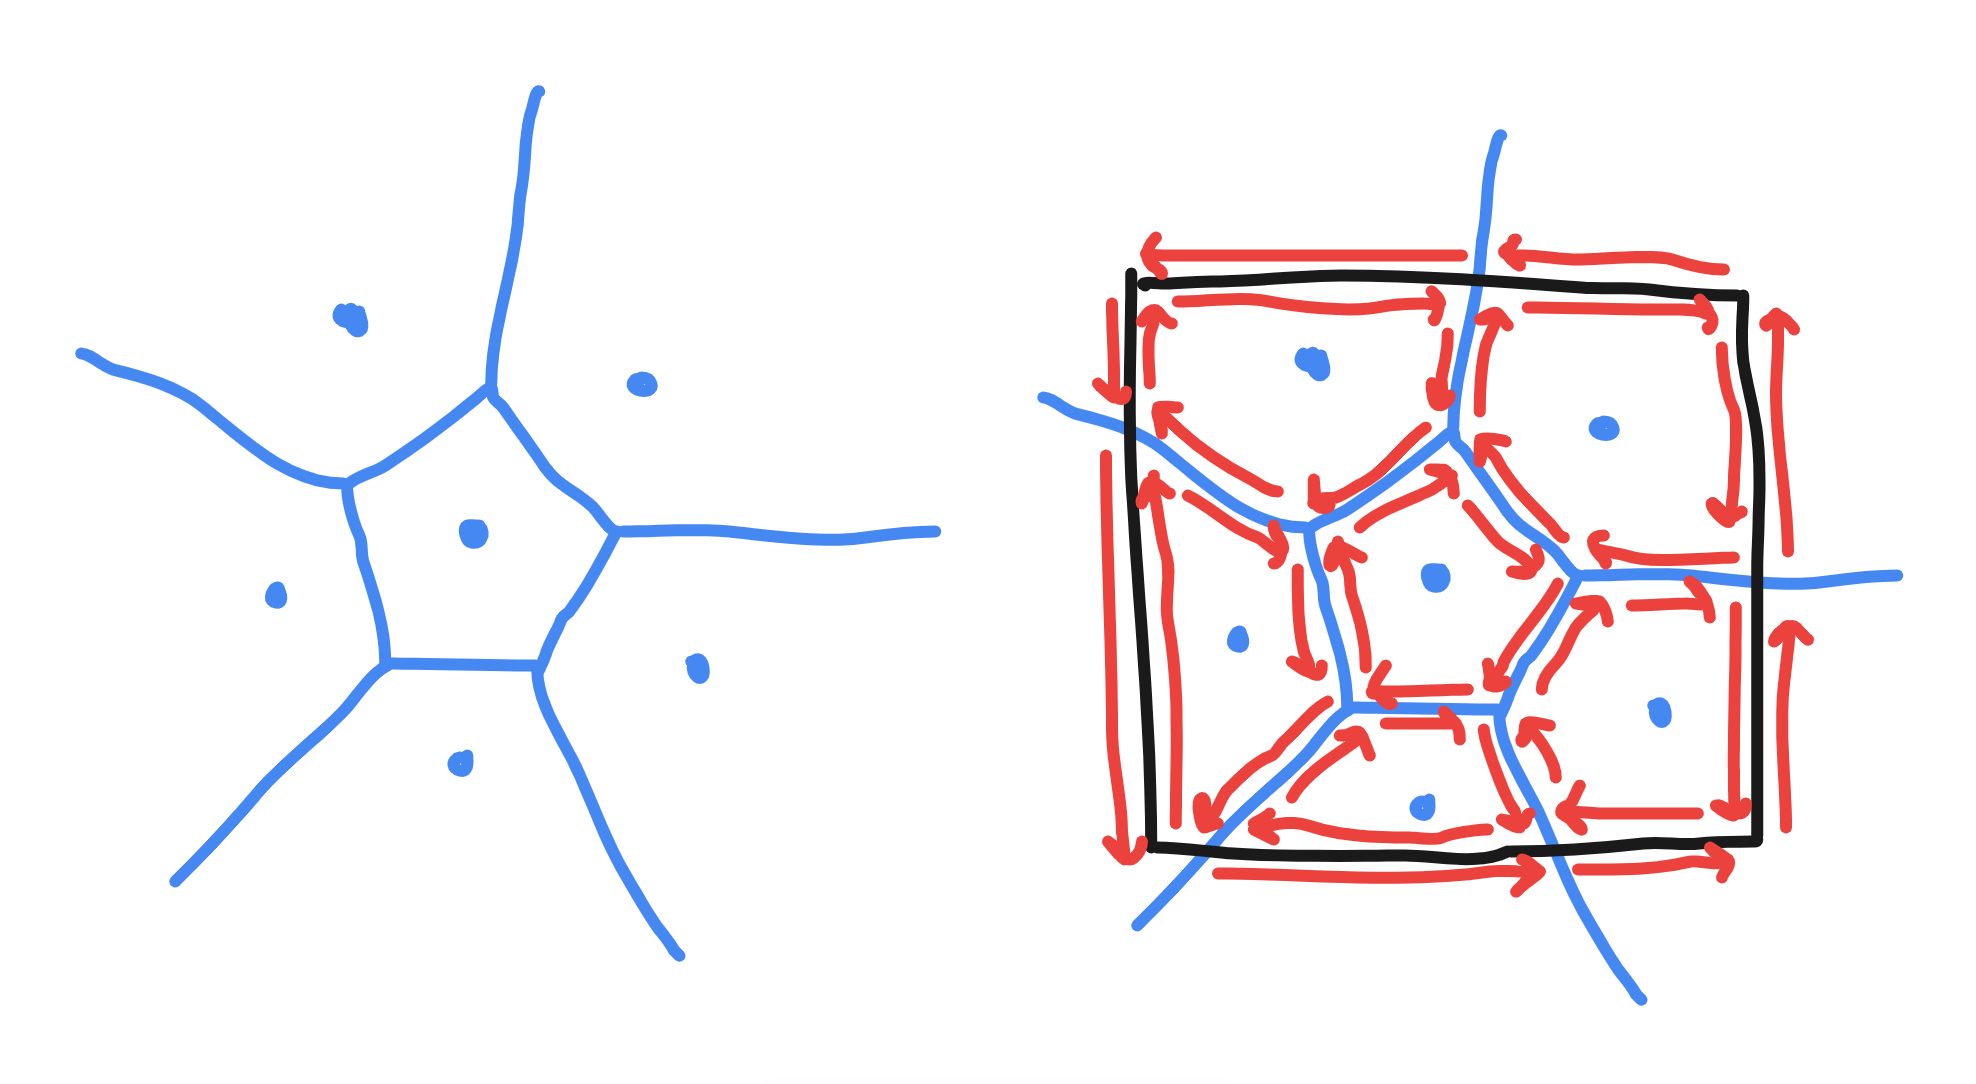
\includegraphics[scale=0.25]{temp-fig-3}
\]
The aim of our algorithms will then be to calculate the DCEL in the right figure.